% Figure 4: the wind-power training trace (P-ALIGN row 118), one row per step, with the key steps
% highlighted. Built at the paper's text width (455pt), so fonts print at their nominal size.
% Compile with: pdflatex key_steps.tex  ->  key_steps.pdf
\documentclass[11pt,border=0pt]{standalone}
\usepackage{times}
\usepackage[T1]{fontenc}
\usepackage{inconsolata}
\usepackage{amsmath}
\usepackage{tikz}
\usetikzlibrary{decorations.pathreplacing}

\definecolor{up}{HTML}{2A78D6}     % categorical slot 1, as in make_figures.py
\definecolor{down}{HTML}{EB6834}   % categorical slot 2
\definecolor{muted}{HTML}{52514E}
\definecolor{rule}{HTML}{B9B8B3}
\newcommand{\eop}{{\scriptsize\texttt{<End\_of\_Prefix>}}}
\newcommand{\law}{$P_w=\tfrac12\rho A v^3$}

\newcommand{\rowh}{12}       % row pitch (pt)
\newcommand{\dotx}{24}       % timeline
\newcommand{\idx}{29}        % step index
\newcommand{\textx}{47}      % step text
\newcommand{\bandr}{322}     % right end of a highlight band
\newcommand{\notex}{328}     % annotation

% \band{k}{color}: highlight behind step k.
\newcommand{\band}[2]{\fill[#2] (\textx-4,{-#1*\rowh-5.6}) rectangle (\bandr,{-#1*\rowh+5.6});}
% \step{k}{text}: index and abridged text of step k.
\newcommand{\step}[2]{%
  \node[anchor=west,inner sep=0pt,text=muted,font=\scriptsize] at (\idx,{-#1*\rowh}) {$s_{#1}$};
  \node[anchor=west,inner sep=0pt] at (\textx,{-#1*\rowh}) {#2};}
% \note{k}{color}{text}: annotation to the right of step k.
\newcommand{\note}[3]{%
  \node[anchor=west,inner sep=0pt,font=\scriptsize\itshape,text=#2] at (\notex,{-#1*\rowh}) {#3};}

\begin{document}
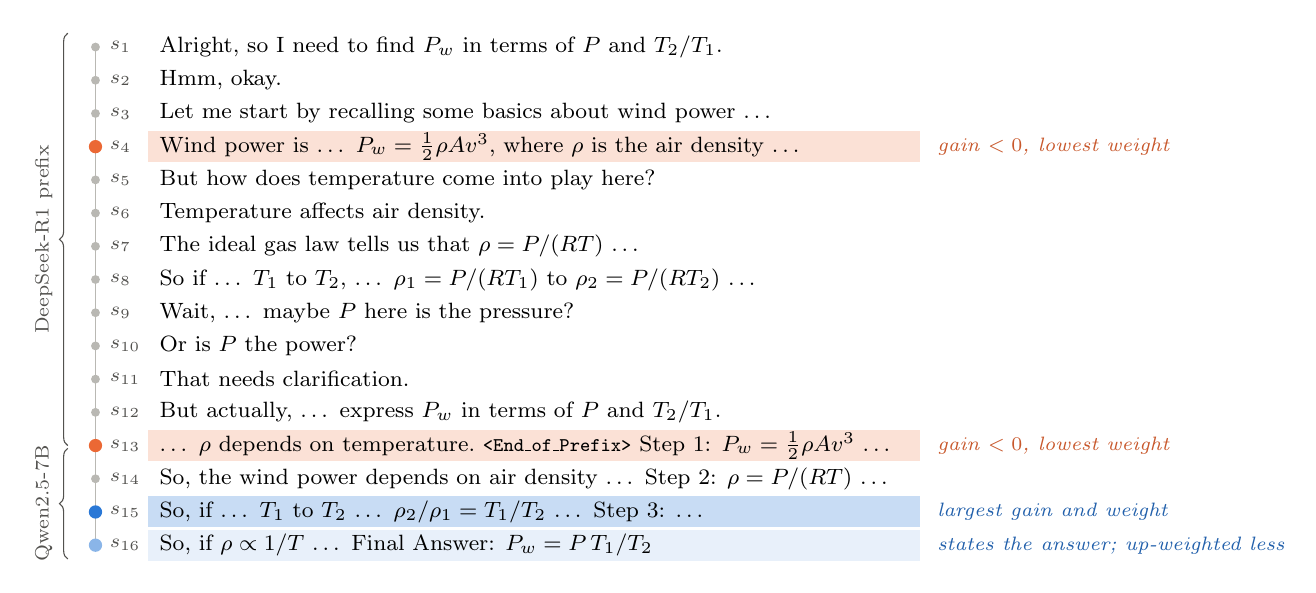
\begin{tikzpicture}[x=1pt,y=1pt,font=\footnotesize]
  % The picture spans exactly the text width.
  \useasboundingbox (-0.5,{-0.5*\rowh+1}) rectangle (454.7,{-16.5*\rowh-1});

  \band{4}{down!20}
  \band{13}{down!20}
  \band{15}{up!26}
  \band{16}{up!11}

  % Timeline; key steps get a colored dot.
  \draw[rule,line width=0.6pt] (\dotx,-\rowh) -- (\dotx,{-16*\rowh});
  \foreach \k in {1,2,3,5,6,7,8,9,10,11,12,14} \fill[rule] (\dotx,{-\k*\rowh}) circle (1.6pt);
  \foreach \k/\c in {4/down,13/down,15/up,16/up!55} \fill[\c] (\dotx,{-\k*\rowh}) circle (2.4pt);

  % Who wrote which steps: the DeepSeek-R1 prefix ends inside s13.
  \draw[decorate,decoration={brace,amplitude=3pt},muted] (14,{-13*\rowh}) -- (14,{-1*\rowh+5})
    node[midway,left=2pt,rotate=90,anchor=south,font=\scriptsize,text=muted] {DeepSeek-R1 prefix};
  \draw[decorate,decoration={brace,amplitude=3pt},muted] (14,{-16*\rowh-5}) -- (14,{-13*\rowh-1})
    node[midway,left=2pt,rotate=90,anchor=south,font=\scriptsize,text=muted] {Qwen2.5-7B};

  \step{1}{Alright, so I need to find $P_w$ in terms of $P$ and $T_2/T_1$.}
  \step{2}{Hmm, okay.}
  \step{3}{Let me start by recalling some basics about wind power \ldots}
  \step{4}{Wind power is \ldots\ \law, where $\rho$ is the air density \ldots}
  \step{5}{But how does temperature come into play here?}
  \step{6}{Temperature affects air density.}
  \step{7}{The ideal gas law tells us that $\rho=P/(RT)$ \ldots}
  \step{8}{So if \ldots\ $T_1$ to $T_2$, \ldots\ $\rho_1=P/(RT_1)$ to $\rho_2=P/(RT_2)$ \ldots}
  \step{9}{Wait, \ldots\ maybe $P$ here is the pressure?}
  \step{10}{Or is $P$ the power?}
  \step{11}{That needs clarification.}
  \step{12}{But actually, \ldots\ express $P_w$ in terms of $P$ and $T_2/T_1$.}
  \step{13}{\ldots\ $\rho$ depends on temperature.\ \eop\ Step 1: \law\ \ldots}
  \step{14}{So, the wind power depends on air density \ldots\ Step 2: $\rho=P/(RT)$ \ldots}
  \step{15}{So, if \ldots\ $T_1$ to $T_2$ \ldots\ $\rho_2/\rho_1=T_1/T_2$ \ldots\ Step 3: \ldots}
  \step{16}{So, if $\rho\propto 1/T$ \ldots\ Final Answer: $P_w=P\,T_1/T_2$}

  \note{4}{down!85!black}{gain $<0$, lowest weight}
  \note{13}{down!85!black}{gain $<0$, lowest weight}
  \note{15}{up!80!black}{largest gain and weight}
  \note{16}{up!80!black}{states the answer; up-weighted less}
\end{tikzpicture}
\end{document}
